\documentclass[12pt]{article}

\usepackage[letterpaper, hmargin=0.75in, vmargin=0.75in]{geometry}
\usepackage{float}
\usepackage{listings}
\usepackage{verbatim}
\usepackage{graphicx}
\usepackage[toc,page]{appendix}

\setlength{\parskip}{8pt}
\pagestyle{empty}

\title{TrueType Font Program Table Tree Shaking}

\author{
  Eduardo Hauck dos Santos\\
  \texttt{eduardohauck@gmail.com}
  \and
  Patrick Lam\\
  \texttt{p.lam@ece.uwaterloo.ca}
}

\lstset{frame=single}

\begin{document}

\maketitle

\section{Motivation}
TrueType is an outline font standard desgined by Apple and Microsoft as
a competitor to Adobe's Type 1 fonts. In TrueType fonts, each glyph is
described by a set of outlines. To ensure excellent font rendering at typical
screen resolutions, font hinting is often used to adjust the display of
an outline. TrueType font hints are expressed in a TrueType-specific
stack-based bytecode language.

With the increasing popularity and spread of TrueType fonts, keeping
them  minimal is a challenge due to the lack of optimizing techniques
for its bytecode. Websites or documents with embedded fonts would benefit
from smaller font files, specially on mobile devices with network or
memory limitations.

TrueType fonts files in the wild often contain bytecode that is never
executed. This work investigates how much we can shrink TrueType font
files if we remove some of this bytecode, specifically, unnecessary
function definitions from the font program table.

\section{Description}

Our tree shaking tool reduces the font program table of a
TrueType font by removing function definitions that are never called
during execution. The output of the tree shake is a new font file with
smaller size if any uncalled functions were identified during tree shaking.

The tree shake can be combined with subsetting techniques to achieve a
better relative reduction from the original size of the font file. Font
subsetting takes a font as input and produces a new font as output,
containing only a subset of the glyphs from the original. It can be used
for webpages or documents whose selection of glyphs remain static after
initial rendering. Subsetting may also remove the need for functions
used by specific glyphs.

To decide which functions can be eliminated, we need to identify the
functions defined and all the function calls made during execution.

Function definitions are located within the font program table in the
form of stack based code. Since this table contains exclusively function
definitions (e.g. no instructions other than function definition
instructions are executed) we can obtain and store their labels
straightforwardly. 

\begin{figure}[ht!]
\begin{verbatim}
PUSH[ ]  /* 2 values pushed */
2 1
FDEF[ ]
PUSH[ ]
14
SWAP[ ]
WCVTP[ ]
ENDF[ ]
FDEF[ ]
DUP[ ]
RCVT[ ]
PUSH[ ]
0
RS[ ]
ADD[ ]
WCVTP[ ]
ENDF[ ]
\end{verbatim}
\caption{Example of a simple font program table}
\end{figure}

Figure 1 shows that by just inspecting the contents (data) of
the PUSH instructions outside of FDEF-ENDF pairs, we can obtain all the
function labels for a font file. Since the program font table only
includes function definitions, we know that the only instructions to pop
elements from the stack are FDEF instructions, and that these elements
will be function labels.

To obtain the function calls, we need to check the bytecode from every
other table, including the bytecode of each glyph. Unlike function
definitions, however, we can not obtain which labels are referred by each
call instruction straightforwardly. That is because CALL instructions
are not necessarily made after a PUSH instruction with the corresponding
label function. The labels can be pushed to the stack anywhere in the
bytecode, although they are usually pushed at the beginning of the
execution. Since every instruction and function call can change the
current state of the stack, when execution reaches a CALL instruction, we
can not be sure about what is the current value at the top of the stack. 

\begin{figure}[ht!]
\begin{verbatim}
PUSH[ ]  /* 3 values pushed */
85 97 93
CALL[ ]
PUSH[ ]
85
CALL[ ]
CALL[ ]
\end{verbatim}
\caption{Example of a program to be executed}
\end{figure}

Figure 2 shows a program with three function calls. The program
initially pushes 3 values to the stack and make the first function call.
We know for sure that the the first function call will refer to the
function labelled 93 because this is the value at the top of the stack
when the first CALL instruction is executed. The same goes for the
second CALL instruction, as the value 85 is pushed immediately before
it. However, for the third CALL instruction, we can not be sure about which
value is at the top of the stack because the second function call may have
changed the state of the stack.  

Therefore, to identify function calls within the bytecode of other tables,
we need to keep track of how many values are pushed and popped by each
instruction and by each function called, so whenever a CALL instruction
is made, we know what is the value at the top of the stack. To achieve
that, we make use of the Abstract Interpreter\cite{bytecode}. Abstract
execution, provides information about the stack height and contents
after each instruction, as well as every possible branch that can be
executed, allowing us to make a list of function calls for each table. 

\section{Background Information}

A TrueType font file is made of tables that contains data comprising an
outline font. A compreehensive list of all the tables that can be
present in a font file can be found in the Apple's TrueType Reference
Manual\cite{ttmanual}. The tables that we are going to focus on this
work are the fpgm, prep and glyf tables. The fpgm is the table that we
are trying to reduce, which contains function definitions. The prep
table contains a set of instructions that are executed whenever the font
is first accessed or when the font, point size or transformation matrix
change. The glyf table contains information that describe glyphs in the
TrueType outline format.

To gather a general idea of how much size each table takes in the font
file, we used the set of TrueType fonts Google Noto Sans\cite{notosans}
to inspect the individual size of each table for a font file. For all
fonts inspected, tables related to glyphs (e.g. glyf, GPOS, GSUB, etc)
take together more than 50 percent of the total size of whole fonts,
while the fpgm table never gets above 10 percent.  

To perform the tree shaking on the font program table,
we make use of related work focused on TrueType fonts, specifically,
the TTFont class present in the fonttools project \cite{fonttools} 
(an open source project) and a bytecode manipulation library
\cite{bytecode} initiated by Wenzhu Man. 

The TTFont class gives us easy access to the TrueType font format. It
allows us to extract data from the font tables, perform analysis on
them, and even manipulate and save them back to the font. 

To get information about rendered glyphs and make sure that
our modifications do not cause any unexpected changes in the font file,
we use the FreeType interpreter to load each glyph from the original
and reduced fonts at a given resolution and make sure they are exactly
the same. 

The Abstract Interpreter can be used to get information about the
program's execution. During abstract execution, instructions do not
return actual values, only abstract data. Although this kind of
execution may offer some limitations compared to normal (concrete)
interpretation, we can estimate  the program's control flow, including
which kind of instructions and functions were called. The Abstract
Interpreter does not run using a TTFont object itself, but instead the
bytecodeContainer class, an intermediate class.

The bytecodeContainer class, as mentioned, is an intermediate of
the TTFont class. It extracts some of the contents of the a font to make
it more easily manipulable and allows translation back to a TTFont
object. The Abstract Interpreter uses a bytecodeContainer, containing 
information about TTFont objects to execute tables of a font.

\section{Disregarding unneeded functions}

The tree shake starts by loading the font file as a TTFont object.
It then create a bytecodeContainer object that encapsulates the main
tables of a TrueType font file: prep, fpgm, cvt and glyf. This object 
is necessary to run the abstract executor. We also create an empty set, 
in which we will insert the labels of functions that were called at some 
point during the execution. This set will be used later on to decide 
which functions we want to keep on the font file.

Whenever a font is loaded, prep is always the first table to run to 
set the environment for glyphs to be loaded. Note that, whenever we run
a table through the Abstract Interpreter, the resulting context
and information about the execution is stored in the interpreter object.
We are interested here specifically in function calls made during the execution.

\begin{figure}[ht!]
\centering
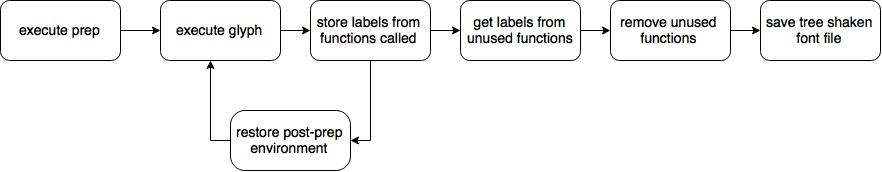
\includegraphics[width=180mm]{diagram.jpg}
\caption{Tree shake diagram \label{overflow}}
\end{figure}

The first step then is running the prep table through the Abstract 
Interpreter. We make a copy of the post-prep environment (we want to be
able to restore this initial state) and update our function label
set with the functions called by prep. We now have everything ready to
execute the remaining tables.

The second step is running every glyph through the Abstract Interpreter.
For each glyph we restore the execution context post-prep, execute the
glyph and update function function call set with calls made during
execution. Afterwards, we have all functions that can possibly be called
by that font.

The third and last step is obtaining the labels of the functions
to be removed (by subtracting the functions called from the list of
functions available in the fpgm table of the font). With them, we update
the bytecodeContainer object --- removing the functions passed --- and
translate the contents of bytecodeContainer back to the TTFont object. 
With that done, the TTFont object is ready to generate a reduced
tree shaken font.

\section{Testing}

To verify that the tree shaking do not interfere with the
renderization of any glyphs, we developed a script to compare glyphs
from two fonts and check if they are identical. While we are using this
script to check if nothing wrong happened during the tree shaking, its
use can be extended to any sort of modification applied to the glyphs of
a TrueType Font.

To perform the comparison, we used the FreeType interpreter to render
glyphs from both fonts (original and reduced) for each charmap present
in the font. Detailed information about how the FreeType interpreter
renders glyphs can be found at the FreeType Reference Manual
\cite{freetypemanual}. 

The script will compare the two fonts for a given set of glyphs at
five popular dpi resolutions: 72x72, 300x300, 600x600, 1200x1200 and
2400x2400dpi. Depending on the number of glyphs to be fetched, and from
where they have to be fetched from (file or URL), the test may take a
while. The default encoding is set to UTF-8. Both resolution and
enconding can also be specified via parameter.

\section{Results}

To measure the results of our work, we performed the tree shaking
technique on the Google Noto Sans fonts\cite{notosans}. To obtain a
better insight on how much the font program table takes in the total
size of the font, we also applied the tree shaking on subsetted fonts
(fetching glyphs from the initial Wikipedia page from the corresponding
languages), to check against the reduction we obtained from the original
fonts.

\verbatiminput{averageStats}

The statistic show a slight variation between the reduction we obtained
with the tree shaking technique for whole fonts and for subsetted fonts.

Although we obtained a better relative reduction for subsetted fonts, the
reduction still averaged under 10 percent. For some fonts, like
NotoSansSinhala-Regular.ttf, the difference in relative reduction
between whole and subsetted font was less than 1 percent, and for fonts
like NotoSansGeorgian-Regular.ttf, this difference jumped to more than
10 percent. Appendix A contains detailed information about every font.

These results give us some insight on how much the function program
table affects the total size of the font, and more importantly, how
other tables contribute to the final size. We could observe that the
reduction we obtained from just subsetting the fonts greatly
varied, presenting reductions between 8 and 99 percent. The tree shaking
yields a better relative reduction in fonts that had their sizes
considerably reduced after subsetting, since the tables related to
glyphs usually take the major part of whole fonts.

Appendix B contains detailed information about how much each table takes
in the Google Noto Sans font files before and after subsetting.

\section{Conclusions and Future Work}

The tree shake of the font program table of TrueType fonts helps to keep
them minimal, which may be useful for further manipulations such as
font merging. However, it proved to be not very efficient for size
reduction.

During our work, we had the chance to investigate the contents
of TrueType fonts, including how much each table takes in the final size
of the font. Our script can obtain such information from fonts in the
wild, which can be useful for further investigation of TrueType fonts.

Possible future works include improvements on the tree shake such as
identifying and removing duplicated functions from the font program
table, as well as the inspection of the other tables to identify
redudant bytecode or the search for new techniques to reduce these
tables.

\clearpage
\begin{appendices}
\section{Tree Shaking Statistics}

\verbatiminput{generalStats}

\section{Table Statatistics}

To understand better how much the subsetting technique would affect
fonts in the wild, we inspected the size of each table before and after
subsetting.

To get information about the size of the tables, we used the TTX tool
from the fonttools project, to dump the font file into an XML file. With
an XML file, we were able to count the number of bytes of each table.

Note that the information we get about sizes are not exact. The size
between the XML file and the original font file may differ, however, as the
results show, this difference is usually reasonably low. Moreover, we
are interested in understanding the relative size of a table when
compared to the other tables in the font. So, even though we are not
getting precise values from an XML file, it is still enough for
understanding how tables compare between each other.

To make sure the glyphs would be rendered the same way as the original
fonts, we used the compare script to check for equality between original
and subsetted for the set of fetched glyphs. 

\verbatiminput{subsetStats}

\end{appendices}

\clearpage
\begin{thebibliography}{1}

\bibitem{fonttools} The fonttools project. {\em https://github.com/behdad/fonttools } 

\bibitem{bytecode} TrueType bytecode manipulation library. 
{\em https://github.com/wenzhuman/fonttools } 

\bibitem{ttmanual} TrueType Reference Manual. 
{\em https://developer.apple.com/fonts/TrueType-Reference-Manual/ } 

\bibitem{freetypemanual} FreeType Documentation.
{\em http://www.freetype.org/freetype2/docs/documentation.html }

\bibitem{notosans} Google Noto Sans. 
{\em https://www.google.com/fonts/specimen/Noto+Sans } 

\end{thebibliography}

\end{document}
